% !TeX spellcheck = pt_BR
% !TEX root = ../main_text.tex
% !TeX encoding = UTF-8
\chapter{Introdução} \label{chap:introducao}
    \todo[inline]{procurar por '?'}
    \todo[inline]{wearables sistemas wearables} % to querendo tudo para ou sistemas ou computação ou dispositivo wearable
    \todo[inline]{SEs}
    
    
    %\todo[inline]{1) Contextualização: Apresente uma visão da área identificando a importância do contexto q está trabalhando. Introduza os "termos" mais importantes.}
    
    %O projeto de Sistemas Embarcados (SE) está cada dia mais complexo \citep{Jozwiak2017}. 
    %
    O recente progresso na obtenção e manipulação de informação, em conjunto com a ascensão das tecnologias microeletrônica, comunicação e sensores proporcionaram um enorme estímulo no desenvolvimento de sistemas computacionais embarcados \citep{Jozwiak2017}.
    %
    A demanda por curto tempo para disponibilidade de produtos ao mercado somado em exigirem propriedades como alto desempenho, baixo consumo de energia e alocação de recursos, representam um desafio para projetistas de sistemas.% \wearables.
    
    % wearable
    Sistemas \Wearables,\ subcategoria de Sistemas Embarcados (SE), possuem o propósito de integrarem-se ao sistema corporal, expandindo suas capacidades e criando uma integração cada vez mais intensa entre ser humano e tecnologia, sendo sua presença não imediatamente óbvia.
    Envolvem múltiplos sensores ou outros sistemas e são requeridos para prover serviço autônomo, contínuo, em um longo período de tempo.
    
    Esses sistemas possuem diversos componentes implementados em \hs\ e ainda é um desafio combinar alto desempenho com baixo consumo de energia maximizando o tempo de uso \citep{Wolf1994, Edwards1994}.
    %
    Uma das maneiras de lidar com tais problemas consiste na combinação das funções do processador/controlador com os recursos dos Arranjo de Portas Programáveis em Campo (FPGAs, do inglês \textit{Field-Programmable Gates Array}) formando um sistema computacional híbrido.
    
    
    %particionamento
    A decisão tomada na escolha de nível de implementação de cada seção de código nesses sistemas é chamada de Particionamento \HS\ (também abreviado como particionamento). 
    Trata-se da escolha onde cada seção de código será implementada sendo ela em nível de \software\ por meio de execução pelos controladores ou em \hardware\ por meio de circuitos digitais dedicados à função e tem-se mostrado promissora aumentando o desempenho destes sistemas \citep{Sass2010, BenHajHassine2017}.
    %
    As pesquisas em \codesign\ de \hs\ têm como objetivo o \design\ de sistemas heterogêneos, visando desempenho, custo e metas de confiabilidade \citep{Edwards1994}.
    
    
    
    
    
    %\todo[inline]{3) Descreva o estado da arte atual, sempre referenciando trabalhos importantes.}
    
    Trabalhos como de \citet{Zhang2008, BenHajHassine2017, Wolf1994, Stone2010} mostram que, uma implementação customizada em \hardware\ pode prover maior eficiência energética e \speedup,\ sendo este a comparação de desempenho à implementações em \software.\ 
    %
    %\todo[inline]{2) Gap: Quais são as questões em aberto, restrições e limitações do estado atual dessa pesquisa.}
    %
    Entretanto, mesmo com vários estudos relacionados à desempenho com particionamento de SE em plataformas FPGA, não há estudos que avaliam a melhoria de desempenho especificamente para \wearables\ em plataformas FPGA.
    
    A motivação é que tal problema que envolve \design\ colaborativo e multidisciplinar, é um passo-chave no \design\ de produtos modernos \citep{Trappey2016}. 
    Com o desenvolvimento de \designs\ mais complexos, esse problema torna-se cada vez mais necessário, no qual o grande requisito para eficiência necessariamente segue junto com a alta velocidade de processamento \citep{Trindade2016, Arato2005, Yan2017}.
    Implementações que baseiam-se somente em módulos em nível de \software\ possuem mais flexibilidade e são menos custosos, entretanto, seu custo eleva-se em termos de tempo de execução. 
    Uma implementação de \hardware\ customizada de um conjunto de instruções proverá uma eficiência energética e \speedup\ maior relativa à implementações em \software\ \citep{Zhang2008, BenHajHassine2017, Wolf1994, Stone2010}.
    
    
    
    %\todo[inline]{4) Propósito+metodologia: Descreva o propósito do seu artigo utilizando para isso uma pitada da sua metodologia.}
    
    Dessa forma, esta pesquisa consiste no particionamento de alguns algoritmos candidatos do \wearable\ comparando o desempenho, alocação de recursos e gasto energético de ambas as implementações \hs.
    %
    % combinação de fpga com cpu
    Ao utilizar o FPGA é possível implementar um sistema e acelerá-lo usando recursos de \hardware\ por meio do particionamento, o que melhora o desempenho e eficiência energética \citep{Cong2009, Lo2009, Zhang2008a}.
    
    
    %\subsection{Contribuição}
    %parece mais objetivo que contribuição
    %Esta pesquisa consiste numa busca sobre o aprimoramento de desempenho de dispositivos computacionais \wearables\ em \hardwares\ reconfiguráveis, utilizando particionamento \hs\ como meio.
    %Visa gastos relativos ao uso de recursos em \hardware\ e gasto energético.
    A principal contribuição deste trabalho é exibir que particionamento \hs\ é uma excelente técnica para a melhoria de desempenho de \wearables,\ como será exibido.
    
    Adicionalmente, algumas contribuições específicas são listadas a seguir:
    
    \begin{enumerate}
        \item 
        %Apresentação da modelagem do problema de particionamento \hs\ aplicando tal técnica nessa classe de sistemas embarcados, buscando pelo aprimoramento de desempenho;
        
        Apresentação de uma modelagem do problema de particionamento aplicado à \wearables,\ buscando maior desempenho;
        
        \item 
        % wearables e particionamento
        %Introdução de sistemas computacionais \wearables\ na qual possuem restrições de consumo energético e recursos, utilizando uma plataforma FPGA como meio para análise de recursos alocados; 
        Utilização de plataforma FPGA em sistemas \wearables\ com restrições energéticas e de recursos;
        
        
        \item %Obtenção de pelo menos $9,6\%$ a mais de desempenho em três de quatros algoritmos avaliados, alocando $5,5\%$ de recursos de \hardware\ reconfigurável e aumento de $ 5,4\% $ de gasto energético;
        Análise de desempenho de quatro algoritmos utilizando particionamento em \hardware\ considerando alocação de recursos e consumo energético.
        
        \item 
        Análise de como as interfaces de comunicação entre \hs\ e otimizações influenciam no desempenho dos \wearables.
        
        %\item Os resultados mostram que com o uso da técnica de particionamento \hs\ em pedaços de código do \wearable,\ aumentou-se o desempenho do sistema pelo menos 2,2\%, chegando até em 41,6\% a mais em desempenho.
    \end{enumerate}
    
    A pesquisa selecionou vários algoritmos do \wearable,\ sendo eles o Estatístico \Ss$_{Es}$, Lagrange \Ss$_{La}$, Números Primos \Ss$_{NP}$ e Risco \Ss$_{Ri}$ e para cada um realizou-se verificações de desempenho e gasto de recursos e energia, e com isso obteve-se uma melhora de desempenho em relação à sua versão em \software\ de 2,2\%, 41,6\%, 9,6\% e 17,8\% respectivamente.
    
    
    
    \section{Organização da Dissertação}
        Os demais capítulos deste trabalho foram divididos da seguinte forma: 
        No Capítulo \ref{chap:revisao_bibliografica} é apresentada uma revisão bibliográfica do problema com informações relevantes para o compreendimento. 
        No Capítulo \ref{chap:relacionados} são descritos alguns trabalhos relacionados ao tema abordado. 
        No Capítulo \ref{chap:design} é apresentado a metodologia. 
        No Capítulo \ref{chap:prototipo} descreve o protótipo e o procedimento de testes.
        No Capítulo \ref{chap:results} exibe e analisa os resultados e o Capítulo \ref{chap:conclu} conclui e apresenta os trabalhos futuros.








\chapter{Referencial Teórico} \label{chap:revisao_bibliografica}

Neste capítulo serão descritos os principais conceitos necessários para o entendimento dos fundamentos do trabalho.%, além de suas tecnologias e metodologias.


\section{\textit{Field-Programmable Logic Device} (FPGA)}

    Microcomputadores e sistemas digitais de sinais são sistemas que seguem instruções especificadas pelo seu \design.
    Segundo \citet{tocci2003sistemas}, a maioria dos sistemas digitais convencionais do mercado atual não são implementados com portas lógicas individuais.
    Em seu lugar, usa-se dispositivos de lógica programável que contêm circuitos para criar funções lógicas digitais.
    Esses dispositivos não são programados da forma convencional seguindo uma lista de instruções estimuladas em suas entradas, mas em vez disso, seu sistema interno é configurado pelo ato de conectar e desconectar de forma eletrônica de pequenos circuitos.

	%lousa branca
	O FPGA de forma geral é um \hardware\ reconfigurável que permite ao \designer\ de SE ter uma lousa branca em que possa implementar \hardwares\ computacionais digitais personalizados tão facilmente como o desenvolvimento de um \software, como ilustra a Figura \ref{fig:rt-board}.
    
    \begin{figure}[h] \centering
        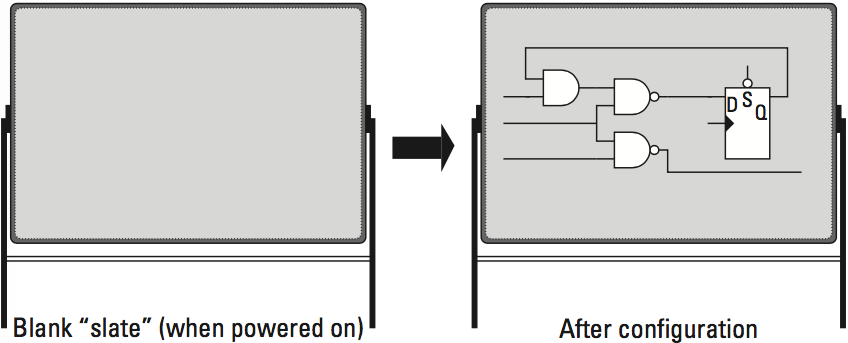
\includegraphics[width=0.9\textwidth]{img/rt-board.png}
        \caption{Ilustração em alto nível do funcionamento interno do FPGA. Fonte: \citet{Sass2010}.}
        \label{fig:rt-board}
    \end{figure}
    
    % o que é um fpga
    %LUTS
    O FPGA constitui-se de vários módulos lógicos pequenos, programáveis, independentes e interconectados para criar funções maiores.
    %Cada módulo lida, normalmente, com até quatro ou cinco variáveis de entrada.
    Utilizam de \textit{Lookup Table} (LuT) para criar as funções lógicas desejadas.
    Uma LuT funciona como uma tabela-verdade onde a saída é programada para representar a função combinacional, armazenando valores verdadeiros e falsos adequado a cada combinação de entrada.
    %Os recursos de roteamento de sinal programável dentro do chip tendem a ser bem variados, com extensões de caminhos diferentes disponíveis.
    %Os atrasos de sinal em um projeto dependem do roteamento real de sinal selecionado pelo \software\ de programação.
    %Os módulos lógicos também contêm registradores programáveis.
    %Eles não são associados a nenhum pino de entrada e saída (I/O, do inglês \textit{Input and Output}).
    %Cada pino de I/O é conectado ao bloco programável de entrada e saída que, por sua vez, é conectado aos módulos lógicos com linhas de roteamento selecionadas.
    Eles reduzem a lista de componentes necessários para o desenvolvimento do projeto, além de simplificar o protótipo, encurtar o ciclo de desenvolvimento e principalmente reduzem o tamanho e os requisitos de potência para o funcionamento do produto \cite{tocci2003sistemas}.
    
    
    
    \subsection{A Tecnologia Reconfigurável e a Plataforma de Manuseio}
    
        %arquitetura
        Uma arquitetura simples de FPGA é exibido na Figura~\ref{fig:rb-arch_fpga}. 
        Nela os quadrados menores situado nas laterais são blocos de I/O que podem ser configurados para fornecer recursos de entrada, saída ou bidirecionais.
        Os quadrados maiores situados no interior são as LuTs, usados para guardar dados que entram ou saem e realizar as operações lógicas.
        Os canais que interligam os blocos entre si são estabelecidas por meio de conexões que passam por linhas e colunas, e possuem a funcionalidade de serem interconexões programáveis \citep{tocci2003sistemas}.
        %A tecnologia interna de um FPGA consiste basicamente de um arranjo de blocos lógicos, canais de roteamento para interconexão de blocos lógicos e blocos de entrada e saída de sinais em torno do circuito.
        Hoje, esses dispositivos possuem milhões de portas de lógica programável, bilhões de transistores, além de outros blocos de \hardware\ dedicados como memórias embarcadas e multiplicadores de ponto-fixo, tornando-o um dos circuitos integrados (CI) mais densos existente \citep{Choi2016}.
        Um projeto terá sucesso de sintetização se ele conseguir ser acordado à quantidade de recursos disponíveis do FPGA e executar rápido o suficiente para concluir seus objetivos sistêmicos \cite{coffman1999real}.
    
        \begin{comment}
        \begin{wrapfigure}{O}{0.5\textwidth} \centering
        %\vspace{-10pt}
        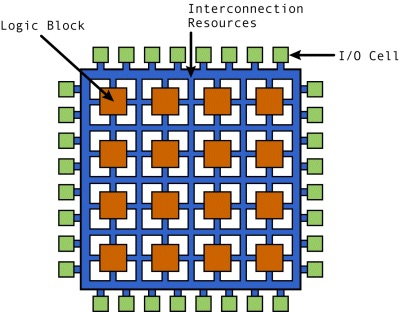
\includegraphics[width=0.5\textwidth]{img/rt-arch_fpga.jpg}
        %\vspace{-15pt}
        \caption{Exemplo em baixo nível da arquitetura internas de um FPGA. Fonte: \url{http://www.eetimes.com/document.asp?doc_id=1274496}. Acesso: 30/05/2018.}
        \label{fig:rb-arch_fpaga}
        \end{wrapfigure}
\end{comment}
        
        \begin{figure}[h] \centering
            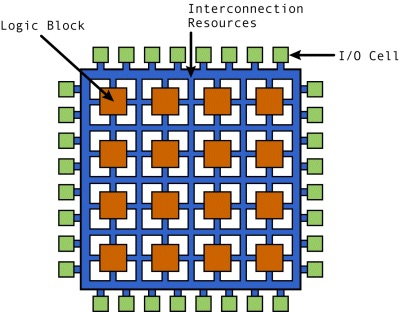
\includegraphics[width=0.65\textwidth]{img/rt-arch_fpga.jpg}
            \caption{Exemplo em baixo nível da arquitetura internas de um FPGA. Fonte: \url{http://www.eetimes.com/document.asp?doc_id=1274496}. Acesso: 30/05/2018.}
            \label{fig:rb-arch_fpga}
        \end{figure}
    
    
    
        % uso de fpga no mundo
        \Hardwares\ reconfiguráveis eram utilizados unicamente na prototipação de projetos de circuitos integrados de aplicação especifica (ASIC, do inglês \textit{Application-Specific Integrated Circuit} e produzido em baixo volume por causa de seu baixo desempenho e custo por unidade.
        Mas com a variedade desses dispositivos disponibilizados hoje no mercado em conjunto com a elevação do custo de pesquisa, \design,\ desenvolvimento e teste e exigências de mercado, houve um crescente interesse na utilização de FPGAs para SE devido suas vantagens sobre ASICs em geral em termos de flexibilidade de projeto e custo e dessa forma dispositivos reconfiguráveis são a tecnologia-chave para o futuro dos sistemas digitais \citep{Mei2000, tocci2003sistemas}.
        
        % Importancia
        \citet{tocci2003sistemas, Plessl2003} citam ainda que o motivo de \hardwares\ reconfiguráveis estarem dominando o mercado é o fato de que, como são dispositivos programáveis, a mesma funcionalidade pode ser obtida ao invés de diversos CI individuais.
        Isso significa maior confiabilidade, menor espaço ocupado na placa, consumo de energia, complexidade de desenvolvimento e, geralmente, menor custo de fabricação.
        
        
    
        % o que é lut
        Ao utilizar a tecnologia \lut,\ o FPGA torna-se versátil para comportar qualquer função digital e também ser eficiente para ser implementado em silício.
        %O controle de entrada de sinais é usado como entrada lógica e o multiplexador de entradas é ligado ao nível lógico para implementar a função desejada \citep{coffman1999real}.
        %
        % o que a sintetização faz
        A ferramenta de sintetização toma o HDL vindo do \designer\ e mapeia-o em \hardware.\ 
        Primeiro o sintetizador irá minimizar equações lógicas removendo termos lógicos redundantes de acordo com seu sistema de optimização e com isso, o \design\ final do projeto será um grande conjunto de equações Booleanas que representa o sistema descrito pelo projetista \citep{coffman1999real}.
       
        
        % tecnologia e energia
        Segundo \citet{tocci2003sistemas}, tais maravilhas de flexibilidade de projetos digitais podem fornecer uma série de opções de projeto sendo voltados para indústria e até mesmo educação.
        Ao utilizar tecnologia como CMOS e SRAM, o consumo de energia do chip é relativamente baixo comparado com outras tecnologias, podendo ser confeccionado em nível de tensão elétrica, frequências e cargas para os sinais de I/O.
        O mercado fornece diferentes FPGAs com graus de velocidade variados a fim de que o projetista utilize o mais adequado ao projeto.
        
        FPGAs rápidos ou com maior número de recursos consequentemente são mais caros e por isso, escolher o FPGA adequado ao projeto também é necessário para obter um bom produto \cite{coffman1999real}.
        %Entretanto, como um dispositivo FPGA pode ser configurado para um número infinito de projetos digitais, isso implica na não possibilidade de afirmar o montante de dissipação de energia para um dispositivo FPGA.
        %O \software\ Quartus II tem duas ferramentas para estimular o montante de uso de energia para uma aplicação.
        %O \textit{PowerPlay Early Power Estimator} é usado durante os estágios iniciais do projeto para estimar a magnitude de potência do dispositivo.
        Dessa forma, FPGAs são chips que podem ser programados instantaneamente para funções de qualquer circuito digital \citep{Choi2016}.
        
        
        
        
        % Plataforma FPGA
        Uma plataforma FPGA é um chip que além de conter o componente FPGA, está integrado à inúmeras interfaces e componentes, desde LEDs (do inglês \textit{Light-Emitting Diode}) e \textit{switchs} até porta Ethernet e interface vídeo VGA (do inglês \textit{Video Graphics Array}) com seus respectivos circuitos.
        Um exemplo de plataforma é exibido na Figura~\ref{fig:rb-arty}.
        Como possui recursos suficientes para circuitos digitais complexos é possível sintetizar por exemplo funções de processamento de imagem, algoritmos de redes de computadores, algoritmos criptográficos e \textit{soft}-processadores completos \citep{Plessl2003}.
        
        \begin{figure}[h] \centering
            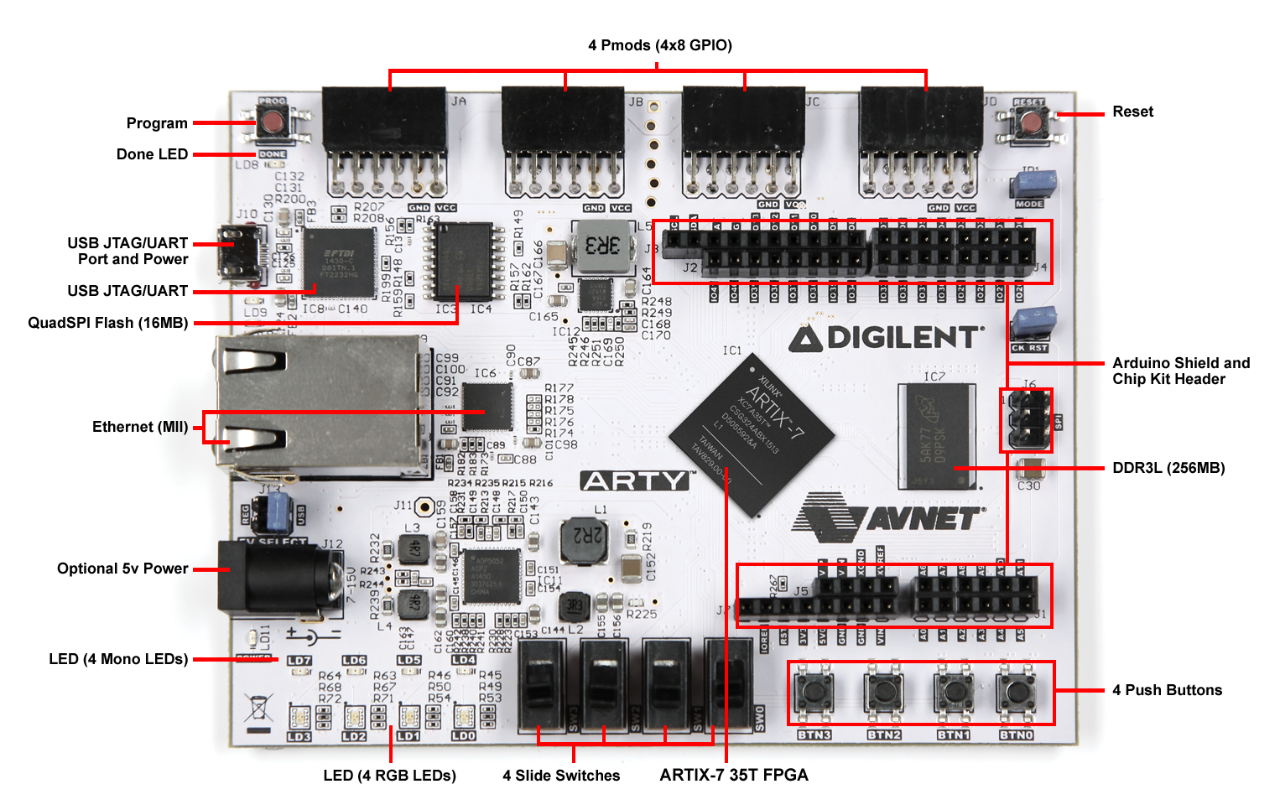
\includegraphics[width=0.99\textwidth]{img/arty.png}
            \caption{Exemplo de uma plataforma FPGA na qual constitui-se de uma placa com o FPGA e seus componentes de interação. Fonte: \url{http://www.xilinx.com/products/boards-and-kits/arty.html}. Acesso: 30/05/2018.}
            \label{fig:rb-arty}
        \end{figure}
   
   
   
    \subsection{Sintetização de Circuitos e Algoritmos no FPGA}
    
    %\subsection{\textit{Hardware Description Language} (HDL)}
        Uma das principais formas de sintetização é utilizando linguagens da classe de Linguagens de Descrição de \Hardware\ (HDL, do inglês \textit{Hardware Description Language}).
        HDL é uma das classes de linguagens de computação usados para descrever formalmente um circuito eletrônico por meio do comportamento temporal ou da estrutura espacial de circuito de um sistema eletrônico, originado pela necessidade de documentar o comportamento do \hardware\ \citep{Sass2010}.
        
        HDL é amplamente utilizada em \design\ de \hardware\ especificando os detalhes de \design\ para qualquer sistema digital, ou seja, tanto para desenvolvimentos de circuitos ASICs quanto para FPGAs.
        Especificado o modelo comportamental de um circuito específico, antes ser projetado e construído, ferramentas lógicas de sínteses são invocadas para gerar informações estatísticas e geométricas que são utilizadas para verificar sua viabilidade.
        %
        Feita as análises, o código é entregue ao compilador lógico chamado de ferramenta de síntese, e sua saída será carregada ao dispositivo reconfigurável, ou seja para suas \luts.\ 
        É possível alterar o código HDL, compilá-lo e fazer sua síntese no mesmo \hardware\ reconfigurável, quantas vezes forem necessárias, sem custo adicional, propriedade única fornecida pela tecnologia da lógica programável \citep{Smith1998}.
        
        Como a maioria dos FPGAs utilizam tecnologia SRAM, eles com isso tornam-se voláteis.
        Isso significa que ao ser energizado, todas as informações de sintetização anteriores se perdem.
        Para contornar este problema, exite também uma memória secundária que guarda as informações de programação que definem como cada bloco lógico comportará, quais blocos serão de entrada e saída, bem como como são as interconexões entre os blocos \cite{tocci2003sistemas}.
                
        Linguagens HDLs como \textit{VHDL} e \textit{Verilog} possuem um nível elevado de complexidade devido suas de naturezas serem linguagem de baixo nível \citep{Choi2016}.
        E para a facilitação do processo de \design,\ existe outra classe de linguagens que permite a sintetização de projetos utilizando linguagens de alto nível \citep{Sass2010}.
        Realizado uma especificação de \design\ em \software, uma Síntese em Alto Nível (HLS, do inglês \textit{High-Level Synthesis}) pode reduzir os longos ciclos do processo de \design\ de \hardware\ e ainda trazer melhoria em desempenho e eficiência energética \citep{Choi2016}.
        Essas linguagens convertem seus códigos em alto nível para HDL e assim realiza-se a sintetização do projeto no \hardware\ reconfigurável.
        
        
        %IP disponibilizados
        Outro item importante na consideração de utilização de FPGA para projetos é a disponibilidade de módulos com propriedade intelectual (IP).
        Este refere-se a projetos predefinidos de módulos complexos usados para satisfazer necessidades de funcionamento do projeto.
        Tais blocos são disponibilizados pelas empresas fabricantes de FPGA ou por fontes terceiras proprietárias destes.
        %
        Dessa forma é possível utilizar módulos completos disponibilizados ou adquiridos a fim de tornar o sistema mais fácil para utilização e robusto.
        Uma variedade de \cores\ IP são disponibilizados para uso em licenciamento barato, na qual são \citep{coffman1999real}:
        \begin{itemize}
            \item Microprocessadores, e \cores\ DSP;
            \item Conversores digitais, GSM e outras formatos e frequências de rádio;
            \item Codificações e decodificações de áudio e vídeo;
            \item Encriptadores e decriptadores PGP e outros algoritmos simétricos e assimétricos;\
            \item DCT, FFT, wavelet e outros cálculos de transformações;
            \item Jogos, \cores\ educacionais e vários outros.
        \end{itemize}
        
        Como o ciclo de vida para produtos está cada vez mais curto por causa do rápido desenvolvimento de tecnologia e recursos, é cada vez mais importante para os desenvolvedores encontrar maneiras de encurtar o ciclo de projeto e desenvolvimento de novos produtos.
        Dessa forma, utilizar de recursos de IP diminuem o tempo necessário ao projetista para concluir seu produto.
    
    
    
    \subsubsection{Otimizações Automáticas de Projeto}
    
        %area e delay optimization
        Segundo \citet{coffman1999real}, a sintetização também realiza otimizações com foco em \textit{delay} e área utilizada.
        O processo é representado como um construtor automático de rotas a partir do HDL, isso é, existe várias formas de fazer a rota de um determinado circuito.
        O processo de sintetização foca em realizar um roteamento que enquadra com os requisitos do \design,\ mesmo se existe a possibilidade de obter melhores resultados em tamanho de área consumida, recursos ou \textit{delay}.
        O resultado da sintetização gerada é avaliada comparando se o sistema gerado é suficiente para ser executado sem erros e isso não significa que o resultado sintetizado gerado será de baixa qualidade pois o \design\ continuará respeitando os requisitos de tempo para seu funcionamento.
        
        Como os conceitos de área e \textit{delay} são inversos entre si, a sintetização mais rápida não buscará ser a menor em espaço e recursos utilizados, da mesma forma que e a busca pela menor área não significará a mais rápida sintetização.
        O quão fácil será a tarefa de sintetização do projeto dependerá de vários fatores como a quantidade de recursos disponíveis do FPGA escolhido para uso, a tecnologia que o FPGA utiliza, os requisitos de velocidade sistêmicos e o \design\ descrito pelo projetista.
    
    
    \subsubsection{Manipulação de Tamanho de Projeto Sintetizável}
    
        %manipulação de tamanho do recurso
        A manipulação do projeto também é passo importante para a quantidade de recursos alocadas a este e qualquer mudança também é substancial.
        Módulos que utilizam grande quantidade de recursos podem ser obter resultados diferentes de sintetização ao quebrar uma rotina em sub-rotinas menores, podendo fazer com que o recurso em \hardware\ fique menor e mais fácil de ser implementado.
        %
        Há três momentos que agregar sub-rotinas também são estratégias inteligentes. 
        Se duas sub-rotinas tomam por exemplo, 25\% cada uma do tempo da aplicação, então elas são fortes candidatas para a implementação em \hardware\ pois usufruem de grande tempo de processamento e este pode ser trabalhado em nível de \hardware. 
        No entanto, se forem implementadas individualmente, cada uma também necessita do custo da sua interface de comunicação com os módulos subsequentes à ela. 
        Se há três sub-rotinas relacionadas (uma invocando a próxima), então a combinação delas pode reduzir o custo de invocações. 
        %Entretanto, o custo da interface não é sempre insignificante e vale a pena o esforço do usuário para investigar a situação.
        
        Da mesma forma, implementações em \hardware\ têm desempenho significativo em usar formatos de dados de dados específicos à sua finalidade. 
        %Para que o \software\ seja mais eficiente nos formato de dados não padronizados, programadores irão investir em estruturas de dados que não são bem mapeadas para o \hardware. 
        Assim, é possível realizar a consideração dos tipos de dados para melhor adaptação ao projeto sintetizado evitando conversões entre níveis \hs\ e com isso explorar melhor o potencial do FPGA visando seu desempenho e recursos utilizados \cite{Sass2010}.
        
        
    \subsubsection{Teste}
        %projedo deve ser pequeno para grande
        O projeto de circuito digital no FPGA deve ser feito a partir do seu modo mais simples, onde escreve-se os trechos de códigos, testá-lo e garantir que ele corresponda à seus requisitos básicos de funcionamento \citep{tocci2003sistemas}.
        
        %teste
        O projetista realiza testes nos módulos construídos visando abordar todos os estímulos possíveis e verificar se a resposta se adéqua às entradas.
        Dessa forma, ao garantir que as pequenas partes funcionam, ao conectá-los, tem-se que o conjunto deles também funcionarão \citep{tocci2003sistemas}.
    
    
    
    \subsection{CSoC}
        É possível também realizar a integração de um controlador/processador à tecnologia FPGA.
        Sistemas que possuem um sistema computacional integrado à uma única placa na qual inclui um FPGA possui o nome Sistema em Chip Configurável (CSoC, do inglês \textit{Configurable System on a Chip}).
        
        Ao utilizar deste sistema, a plataforma FPGA será constituída de uma arquitetura semelhante à exibida na Figura~\ref{fig:rb-soc} onde as setas representam os barramentos de comunicação entre os principais componentes.
        
        \begin{figure}[h] \centering
            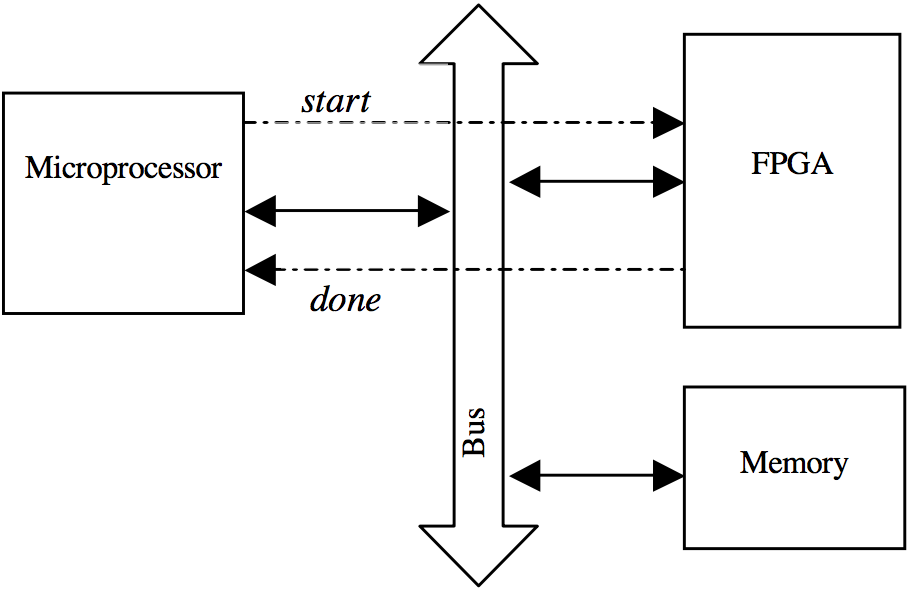
\includegraphics[width=0.7\textwidth]{img/into-soc.png}
            \caption{Visão geral de um SoC FPGA.}
            \label{fig:rb-soc}
        \end{figure}
    
    
        % Utilização de um processador sintético ou físico
        A unidade de processamento central nesses tipos de sistemas pode ser utilizada/implementada de duas formas, sendo estas \textit{hard} e \textit{soft} \cores.
        %
        %hard
        O processador \textit{hard core} é um \core\ fisicamente dedicado. Isso significa que é um um pedaço de CI que pode estar dentro do próprio circuito de um FPGA ou integrado à sua plataforma de componentes na qual possui um barramento para a comunicação.
        Este sistema não utiliza de recursos do FPGA para a utilização do processador.
        %soft
        Já o processador \textit{soft core} é implementado por meio da sintetização e mapeamento de um modelo de um processador no FPGA.
        Dessa forma, ao invés de ter um circuito de um processador independente dos componentes da plataforma, tem-se a sintetização deste dentro do FPGA por meio das \luts.\ 
        Assim, o FPGA deve realizar a construção do sistema completo utilizando seus recursos de construção de circuitos digitais na qual passam pelo mesmo processo das demais sintetizações sendo elas \design\ mapeamento e sintetização na placa.
        
        Cada um tipo de \core\ possui suas vantagens.
        Ao utilizar um \textit{hard} \core, é possível utilizar todos seus recursos obtendo máximo desempenho nas atividades executadas, a utilização de um \textit{soft} \core\ permite a extensão da arquitetura \citep{Plessl2003}.
    
    
        \subsubsection{Processadores \textit{Soft Core}}
        
            %geral
            Devido ao grande aumento do número de microprocessadores na qual podem ser integrados em vários SoC de grande porte que necessitam de robustez, percebeu-se que havia a necessidade de microprocessadores modificáveis. % \citep{kranenburg2010mb}.
            %
            Com o aumento da capacidade dos FPGAs foi possível a construção desses componentes tanto comerciais quanto \textit{open source} em sistemas SoC, utilizados em aplicações que variam desde computação paralela até rede de computadores \citep{kranenburg2010mb}.
            
            % hard e soft
            Um processador \textit{hard core} fabricado não possui nenhuma forma de reconfiguração da lógica de seus dispositivos ASIC.
            Qualquer mudança necessária num projeto desses dispositivos seria necessário realizar uma nova construção da máscara litográfica e uma nova fabricação deste, processo longo e custoso.
            E também quando o sistema baseado em processador com suas instruções customizadas já foi mapeado em um ASIC, a única possibilidade de mudança da aplicação deveria ser realizada em nível de \software,\ alterando seu código.
            %
            Já processadores \textit{soft cores} integram a instrução customizada completamente em suas unidades de execução e são úteis se um determinado \hardware\ não é moldável como são os ASICs.
            Utilizando FPGA como meio para esses SoC nos permite a reconfiguração da lógica interna de forma fácil rápida e barata, isso em qualquer estágio de construção do projeto \citep{rosinger2004connecting}.
        
            % vantagens do soft
            Uma das vantagens do uso de um processador \textit{soft core} é a sua flexibilidade.
            Essa propriedade de projetos de nível alto permite que projetista utilize apenas os recursos realmente necessários do processador para sua aplicação específica.
            Além disso, essa característica também permite que esses processadores sejam facilmente integrados com módulo de IP resultando num processo mais rápido no desenvolvimento de um projeto e um produto final sólido \citep{rosinger2004connecting}.
        
        
        
        
            %microblaze
            MicroBlaze\texttrademark\ é uma família de configurações comerciais predefinidas de um RISC de 32 bits utilizados como módulo IP em desenvolvimento de projetos em FPGA com \textit{soft}-processadores. 
            Ao adicionar o processador ao projeto, é possível utilizar \softwares\ de desenvolvimento que não necessitam de experiência prévia em \hardware\ reconfigurável para desenvolver aplicações para o processador MicroBlaze. 
            O processador MicroBlaze atende aos requisitos de diversas aplicações, incluindo os mercados Industrial, Médico, Automotivo, Consumidor e de Comunicações pois ele possui configurações que suportam o comportamento para classes de processadores em tempo-real, para aplicações em geral e microcontrolador.
            
            % arquitetura
            Ele possui um conjunto de instruções de 32-bit e registradores de propósito geral, além barramento de 32-bits, expansível par 64.
            É possível também incluir unidade de ponto flutuante, permitindo o uso do processador adequando melhor ao projeto.
            Possui suporte à \textit{pipeline} na decodificação de instruções, bem como suporte à interface de comunicação AXI \citep{obeidat2011microblaze}.
            
            
            %microblaze e open source
            Diferentemente de processadores \textit{open source}, MicroBlaze possui qualidade no componente disponibilizado, suporte e documentação disponíveis para o desenvolvedor.
            Muito dos \designs\ \textit{open source} são difíceis de serem modificados devido sua complexidade, além da falta de uma metodologia de \design\ ou a ausência de documentação clara.
            Além de que muitos destes processadores não são portáveis e funcionarão em modelos específicos de FPGAs.
            %
            Processadores comerciais são constantemente escolhidos para uso devido ao fato de terem um preço relativamente barato ao concorrentes e que estes podem ser facilmente acoplados à um projeto sintetizável em FPGA \citep{kranenburg2010mb, kranenburg2009reference, rosinger2004connecting}.
            
            Também é possível construir uma arquitetura básica de um MicroBlaze multi core.
            Instancia-se vários MicroBlazes cada um com memória local privada e todos conectados ao barramento \textit{Open Core Protocol} (OPB) e com isso cada processador tem uma conexão \textit{full-duplex} com os outros MicroBlaze, e uma descrição da arquitetura é exibida na Figura~\ref{fig:rb-multi}  \citep{xu2008multi}.
            
            \begin{figure}[h] \centering
                %\vspace{5pt}
                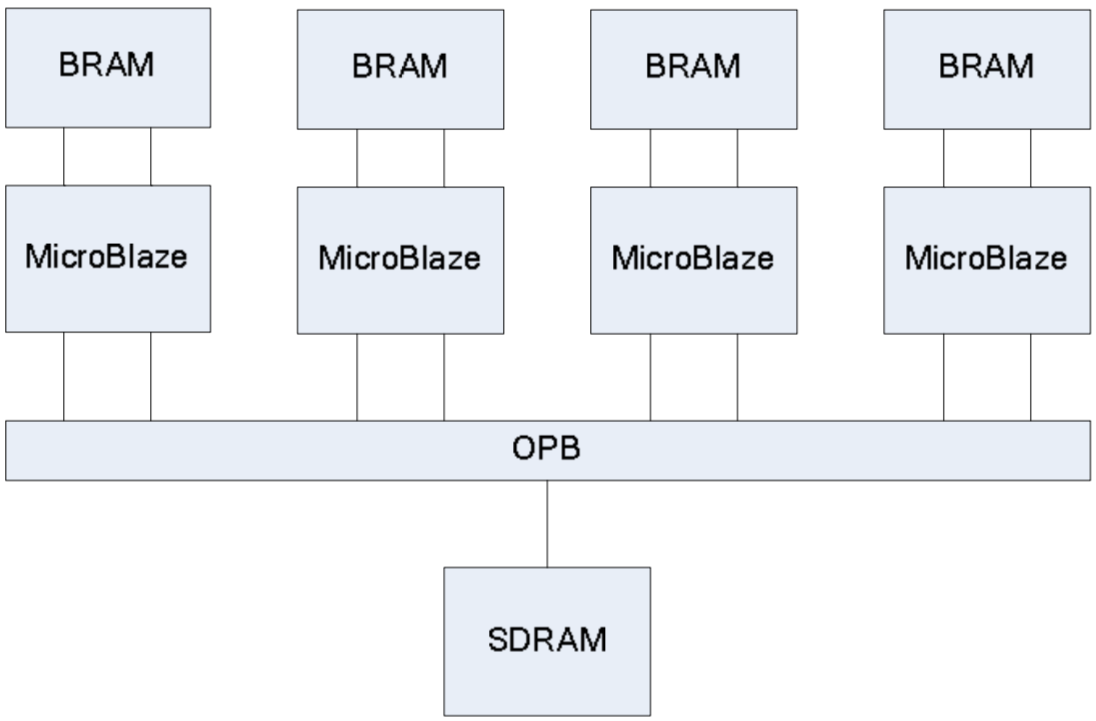
\includegraphics[width=0.7\textwidth]{img/rb-multi-microblaze.png}
                %\vspace{15pt}
                \caption{Esquema de multi-MicroBlazes. Fonte: \citep{xu2008multi}.}
                \label{fig:rb-multi}
            \end{figure}
            
            
            Há diferentes formas de conectar um módulo IP em um processador \textit{soft core}.
            Cada aplicação pode ser realizada e implementada tanto como um algoritmo em \software\ quanto num \hardware\ estrutural como é exibido na Figura~\ref{fig:rb-mb-hs}.
            Neste exemplo, uma mesma porção de código implementado tanto em \hs\ possui diferentes desempenhos.
            Ao utilizar uma implementação em \software\ tem-se seu código sequencial executado pelo processador e na transformação deste em um módulo de \hardware\ pode executá-lo como um módulo dedicado e ainda aplicar otimizações de \hardware\ \citep{rosinger2004connecting}.
            
            \begin{figure}[h] \centering
                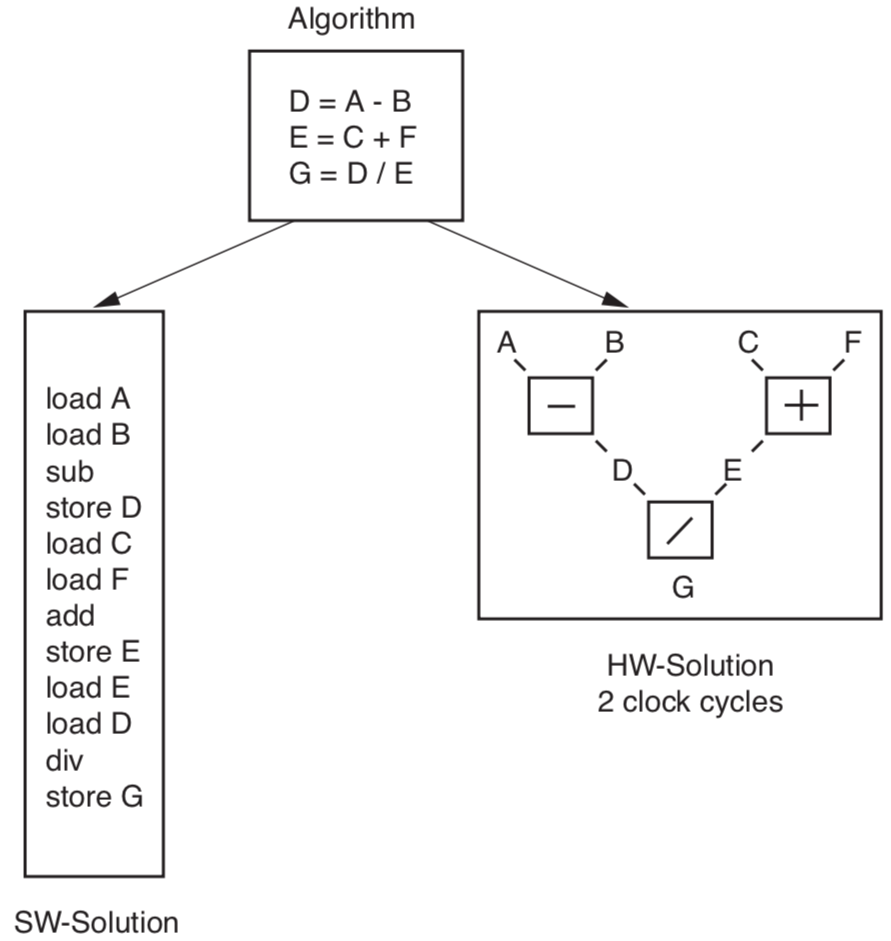
\includegraphics[width=0.67\textwidth]{img/mb-hs.png}
                \caption{Comparação hipotética de implementações em \software\ e \hardware\ com otimizações.}
                \label{fig:rb-mb-hs}
            \end{figure}
            
            Este também permite ao usuário escrever \textit{firmwares} customizados em Verilog e VHDL que atribui ao processador um barramento local permitindo que o projeto possua interface de comunicação com quase todos os dispositivos conectados como sensores, atuadores, sistemas heterogêneos providos externamente \citep{kranenburg2010mb}.
        
            Ao adicionar o processador \textit{soft core} MicroBlaze junto do barramento AXI, o projeto assistido pelo computado será semelhante ao circuito digital exibido pela Figura~\ref{fig:rb-mb}.
            Exibe-se os blocos formados por módulos IP e seus componentes complementares necessários para o funcionamento básico do projeto como memórias e \textit{clocks}.
            
            \begin{figure}[h] \centering
                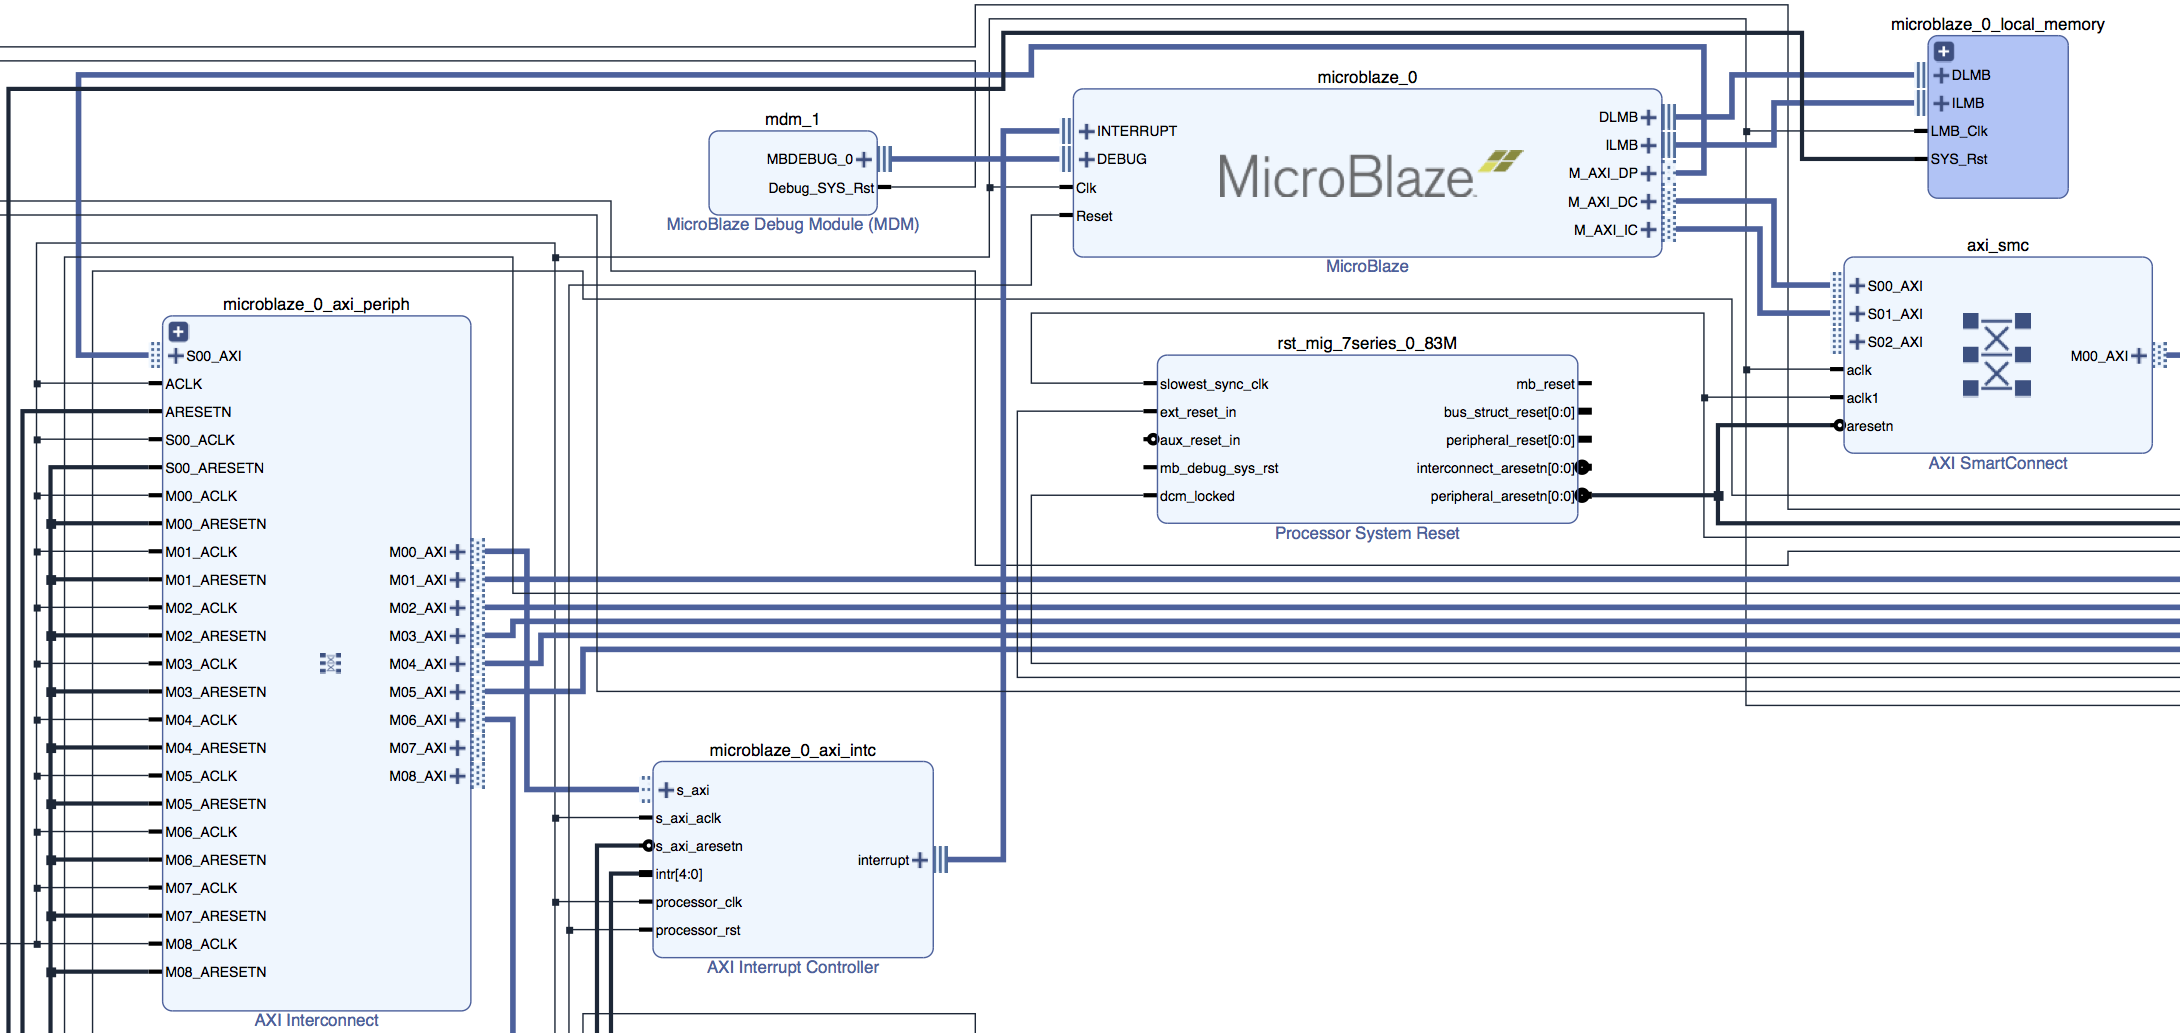
\includegraphics[width=1.0\textwidth]{img/1-microblaze-axi.png}
                \caption{Visão geral do MicroBlaze com o barramento AXI já integrado ao projeto.}
                \label{fig:rb-mb}
            \end{figure}
        
        



\begin{comment}
\section{\Profile} \label{sec:profile}

		\Profile\ é uma procedimento para auxiliar o usuário a coletar informações do \software\ em tempo de execução.
      Existem vários programas diferentes para adquirir essas informações e podem ser distinguidos em duas categorias.
      A primeira é aqueles que apresentam a quantidade de declarações e invocações de rotinas, e aqueles que exibem informações de tempo de declarações e rotinas \citep{nemeth2004manual}. Um exemplo de saída é exibida a seguir.

{ \footnotesize
      \begin{verbatim}
Flat profile:

Each sample counts as 0.01 seconds.
  %   cumulative   self              self     total
 time   seconds   seconds    calls  ms/call  ms/call  name
 33.34      0.02     0.02     7208     0.00     0.00  open
 16.67      0.03     0.01      244     0.04     0.12  offtime
 16.67      0.04     0.01        8     1.25     1.25  memccpy
 16.67      0.05     0.01        7     1.43     1.43  write
 16.67      0.06     0.01                             mcount
  0.00      0.06     0.00      236     0.00     0.00  tzset
  0.00      0.06     0.00      192     0.00     0.00  tolower
  0.00      0.06     0.00       47     0.00     0.00  strlen
  0.00      0.06     0.00       45     0.00     0.00  strchr
      \end{verbatim}
      \vspace{-3em}
}

      \begin{wrapfigure}{o}{0.56\textwidth} \centering
         %\vspace{15pt}
         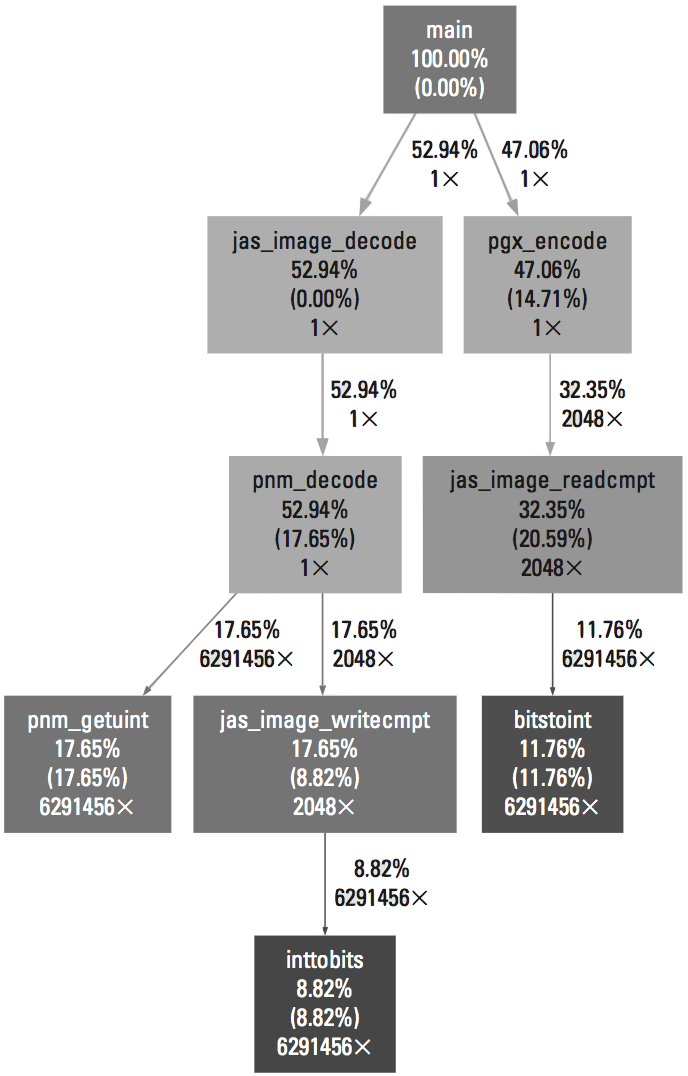
\includegraphics[width=0.48\textwidth]{img/f4-1-2.png}
         %\vspace{-1em}
         \caption{\Profile\ da codificação de imagem em formato JPEG. Fonte: \cite{Sass2010}. \vspace{-0em} }
         %\vspace{-3em}
         \label{fig:profile}
      \end{wrapfigure}

      A Figura \ref{fig:profile} exibe um exemplo gráfico de \profile\ de \software\ em um codificador de imagem em formato JPEG.
      O processo é feito ao colocar o \software\ referencial (programa a ser coletado) como entrada representativa na ferramenta e a coleta é realizada em várias partes da aplicação ao longo de sua execução neste.
		Uma das técnicas do \profile\ de mensurar uma aplicação é na realização de interrupções periódica no programa e amostrar o seu \textit{program counter}.
      Dessa forma, é possível utilizar um histograma para contar quando um programa é interrompido em um endereço particular e a partir dessa informação, calcular a fração aproximada do tempo total de execução gasto em suas partes.
      Distribuições GNU/Linux possuem a ferramenta \texttt{gprof} na qual avalia procedimentos enviados por parâmetro, realizando o cálculo de tais informações de \software\ \citep{Graham1982}.
\end{comment}



\section{Sistemas Computacionais \Wearables}

    %\subsection{Definição}
    
        \citeauthor{starner1996human} em \citeyear{starner1996human} descreveu sistemas computacionais \wearables\ como sistemas que são caracterizados pela sua habilidade de reconhecer o ambiente ao seu redor e comportamentos de seus usuários bem como a situação que os envolvem, e que com esse nível de acesso à informação computacional, revolucionará como os computadores seriam usados.
        Mesmo que esses sistemas ainda eram volumosos e inconvenientes por conta de vários fatores, vários cientistas sustentam essa definição base sobre dispositivos \wearables.\ 
    
        %computadores acoplado ao corpo
        %introdução de que são cheio de sensores e atuadores
        Segundo \citet{Amorim2017, billinghurst1999wearable}, sistemas computacionais \wearables\ são sistemas que com a possibilidade de ter um computador acoplado ao corpo, proporcionam ao usuário um nível superior de informações contextualizadas dentro de um ambiente interativo, podendo ser qualquer dispositivo desde sistemas integrados ao pulso do usuário até mochilas com computadores embutidos.
        Ou seja, são sistemas carregados de sensores e atuadores, acoplados ao corpo, e que proveem medição contínua de parâmetros fisiológicos do usuário ou do seu ambiente ao redor \citep{son2014multifunctional}.
        %
        %deve ser usado em roupa
        % locais que podem ser usados
        %tipo de informações coletadas
        \citet{arias2015privacy} cita que a tecnologia \wearable\ utiliza do pressuposto que deve ser usada em roupas ou acessórios e faz parte de um grande movimento também referenciado como auto quantificado (do inglês \textit{quantified self}).
        Isso refere-se ao autoconhecimento através de números, propriedade permitida pelo seu uso.
        
        Definições mais formais como a de \citet{Gemperle1998} diz que um produto só pode ser considerado \wearable\ se ter a propriedade chamada `\textit{wearability}', sendo esta definida como a interação entre o corpo humano e o objeto \wearable\ estendendo-o em movimento devido à necessidade de movimentação do usuário.
        Esta mesma propriedade está relacionada a objetos mundanos que usamos cotidianamente como roupas e acessórios que não são inteligentes.
        %
        \citet{VanLaerhoven2002} afirmam que a distribuição de elementos computacionais como sensores em objetos mundanos em nosso cotidiano adéqua-se à pesquisa denominada por computação ubíqua e que isso também aplica à computação \wearable,\ uma vez que superfícies de roupas também pode ser uma plataforma de suporte ideal para uma grande quantidade de sensores sendo que estes devem ser miniaturizados para que eles não obstruam seu usuário em seu uso.
        %
        Já \citet{Jozwiak2017} define e caracteriza um sistema computacional \wearable\ como um sistema \textit{cyber}-físico móvel autônomo.
        Em outras palavras \textit{cyber-} é uma combinação dos termos `dispositivo computacional', `rede de computadores' ou `realidade virtual' com um segundo termo, no caso o `físico' oriundo de circuitos.
        
        
        
        %falando + de sensores e atuadores
        Sensores provem um sistema nervoso para detectar sinais.
        Para dispositivos \wearables\ passivos, a existência de sensores é essencial.
        Já atuadores agem uma vez detectado sinais de forma autônoma ou a partir de uma unidade central de controle e assim sendo elementos essenciais para um dispositivo inteligente ativo \citep{starner1996human}.
        %
        Isso significa que tais dispositivos registram e reportam informações sobre o ambiente situado, podendo ser desde avaliação de atividades físicas até padrões de sono.
        Esses dispositivos podem educar e motivar indivíduos a fim de terem melhores hábitos, saúde e segurança, por exemplo \citep{patel2015wearable}.
        %
        As informações coletadas podem variar desde um simples batimento cardíaco e dados de temperatura e umidade até dados sensíveis como a localização atual do próprio usuário e seus hábitos cotidianos de vida.
        
        
        %sistema wearable
        É exibido na Figura~\ref{fig:into-wearable} uma ilustração de um sistema \wearable\ hipotético composto por vários itens como 
        sensores espalhados em seu corpo que ao movimento do usuário são estimulados e geram informações à central, ou 
        componentes atuadores \textit{piezo-electric} integrados ao sapato energizando o sistema \wearable\ com o caminhar \citep{VanLaerhoven2002, Kern2002, Kymissis1998}.
        
        \begin{figure}[h] \centering
            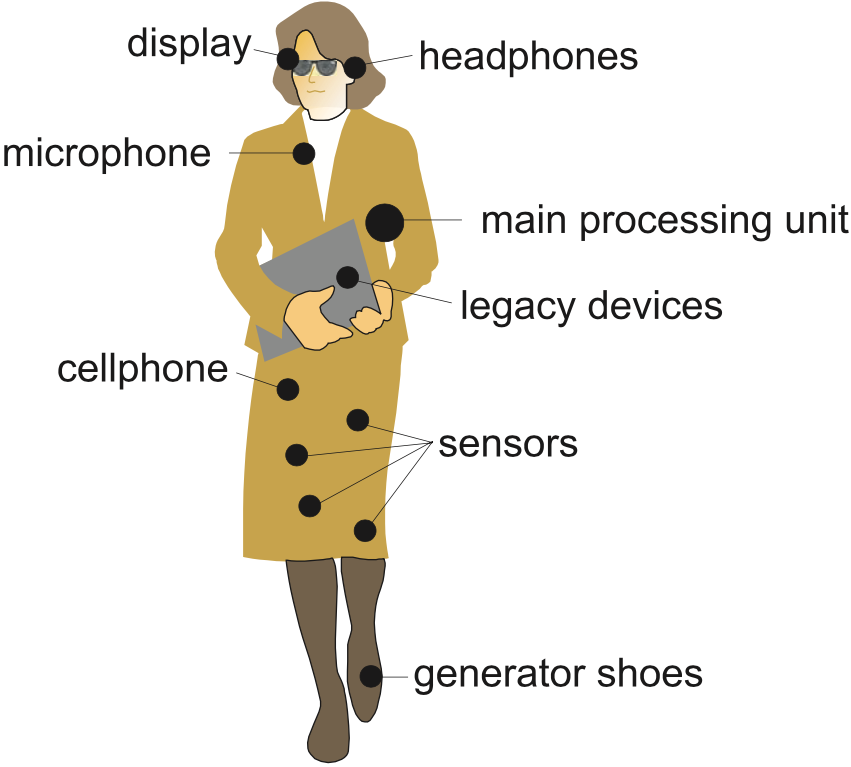
\includegraphics[width=0.66\textwidth]{img/into-wearable2.png}
            \caption{Exemplificação de alguns tipos de dispositivos \wearables.\ Fonte: \citet{Plessl2003}.}
            \label{fig:into-wearable}
        \end{figure}
        
        
        
        \begin{comment}
        %desempenho
        Sistemas \wearables\ executam de tarefas de computação intensiva que consideram restrições de tempo-real onde não realizando-as, o sistema torna-se inaplicável.
        Assim, requere-se um desempenho que seja viável para a execução de suas tarefas.
        % energia
        Da mesma forma, é essencial em um sistema manter-se ativo e funcional num certo período de tempo.
        O \design\ do gasto de energia de um sistema conduz inúmeros desafios e gerenciar esse gasto energético também é um item a ser considerado na construção de um produto.
        Ao alterar os padrões de desempenho de um sistema, seu padrão energético também é alterado \citep{Plessl2003}.
\end{comment}
     
    
    \subsection{Características Funcionais de um \Wearable}
    
        A caracterização de um dispositivo computacional \wearable\ é feita acordando as classificações pré-estabelecidas relacionadas à suas funcionalidades e requisitos de \hardware.
        
        O mercado possui um número considerável de dispositivos \wearables\ que são utilizados em inúmeras áreas, e mesmo que cada equipamento separado tenha suas próprias características, muitas soluções em \hardware\ compartilham uma arquitetura e organização interna de recursos implementados comum.
        Esses detalhes também podem ser expandidos às características relativas à recursos de sistemas operacionais, no qual dispositivos \wearables\ podem ser classificados além de seus componentes de \hardware\ internos como suas funções de desempenho \citep{Delabrida2016, Amorim2017}, como representado pela Figura \ref{fig:classification}.
        
        \begin{figure}[h] \centering
            %\vspace{5pt}
            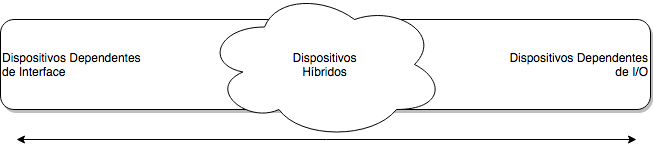
\includegraphics[width=0.97\textwidth]{img/rt-gradiente.png}
            %\vspace{15pt}
            \caption{Classificação de sistemas \wearables. 
                De um extremo existe os dispositivos dependentes de interfaces de usuário e do outro os dependentes de entrada e saída de sinais enquanto entre eles, a gama de combinações possíveis. Fonte: Adaptado de \citep{Amorim2017}.}
            \label{fig:classification}
        \end{figure}
        
        De um lado existem os dispositivos dependentes de interfaces de usuário que possuem alta dependência de operações que fazem referência à comunicação de informação e interação ao usuário sobre sua situação, dessa forma, tais dispositivos provê respostas sobre as interações do usuário.
        Focam principalmente em tarefas para renderização em \textit{displays} como por exemplo equipamentos de realidade virtual e aumentada para implementação de objetos tridimensionais.
        
        De outro lado, existem os dispositivos dependentes de entrada e saída de sinais. 
        Atuam principalmente com o estímulo por algum dado oriundo de outro dispositivo ou do ambiente situado, enviando este dado interpretado à uma nuvem respeitando restrições de tempo-real.
        Isso se da pela utilização de sensores acoplados ao \wearable\ que podem exigir uma boa vazão de dados e pequena latência como são os monitores de atividade remota, situação na qual cria-se o ambiente perfeito para o termo conhecido por IoT (do inglês \textit{Internet of Things}).
        
        Entre dispositivos dependentes de interfaces de usuário e dispositivos de entrada e saída de sinais existe os dispositivos que possui a característica de serem híbridos. 
        São dispositivos que sua natureza é executada sobre características de ambos os extremos citados.
        Dispositivos como \textit{smartwatches} e \textit{fitness trackers} são exemplos de tais dispositivos híbridos, onde possuem restrições de equalização à prioridade dada pelo dispositivo para ambas as operações de interface com o usuário e manipulação de sinais de entrada e saída.
        
        A separação dos conceitos computação \wearable\ e IoT ainda não estão claros segundo a bibliografia científica.
        Sistemas operacionais de propósito específico para ambientes \wearable\ são comumente focado em um único tipo de seguimento de produto como os \textit{smartwatches}, sendo que proporciona aos desenvolvedores um meio para sua aplicação final além de entregar um produto de alta qualidade.
        Também, atualmente, não existe nenhum sistema que satisfaça todos os requisitos apresentados \citep{Amorim2017}.
        
        

    
    \subsection{Miniaturização e Consumo Energético}
    
        %introdução
        O meio científico já estuda \wearables\ há várias décadas como é reportado em trabalhos científicos de \citet{Sutherland1968}, \citet{Mann1996} e \citet{Mann1997}.
        Entretanto, sua comercialização só foi realizada após a miniaturização dos componentes eletrônicos bem com a melhoria na eficiência energética dos mesmo.
        Esse fenômeno fica claro na percepção do crescente espaço ganho recentemente pelos \textit{smartwatches}, \textit{fitness trackers}, óculos inteligentes, equipamentos de realidade virtual e aumentada e outros nas indústrias e nas atividades pessoais de usuários.
        
        %tamanho e qualidade
        Essa restrição de tamanho geralmente significa que a própria qualidade do equipamento também está comprometida, o que leva ao projetista utilizar de muitos atuadores e sensores simplistas no \design\ de um novo produto \citep{VanLaerhoven2002}.
        
        Dispositivos móveis necessitam de sistemas de energização inteligente para seu funcionamento.
        %
        Entretanto, baterias adicionam ao seu projeto tamanho, peso e inconveniência.
        Sobre isso, várias pesquisas foram realizadas de forma a aproveitar o consumo de energia para que o produto possa operar por um período de tempo maior e com a interação mais fluída com o usuário \citep{starner1996human}.
        
        
        Também existe sistemas \wearables\ que são construídos por meio de \textit{electronic textiles}, também conhecidos como, \textit{e-textiles} na qual são fabricações que interconectam eletrônicos em tecidos.
        É possível entregar um produto fisicamente flexível e um tamanho que tipicamente não pode ser alcançado facilmente com outras técnicas de fabricação eletrônicas.
        Com esse tipo de construção, os componentes e suas interconexões são menos visíveis e não suscetíveis a se emaranhar em objetos ao seu redor ou atrapalhar a experiência do usuário.
        Também são facilmente adaptados às rápidas mudanças em tecnologias computacionais e sensoriais de aplicações específicas \citep{starner1996human}.
        
        
        %Comunicação
        Como seu sistema pode ser composto por um conjunto de nós distribuídos, utiliza-se de uma rede de comunicação centralizada num módulo principal realizando a troca de informações entre esses dispositivos.
        Quanto mais dispositivos e componentes como sensores e atuadores conectados no projeto, mais a comunicação torna-se necessária para projeto do sistema e consequentemente mais complexo ele fica.
        Com isso, tem-se então um computador embarcado em um ambiente \mobile\ interagindo com o ambiente ao seu redor, e caso o sistema possua vários nós, a comunicação sem-fio tende a ser a tecnologia predominante por causa da necessidade de mobilidade \citep{Plessl2003,VanLaerhoven2002, Kern2002, Kymissis1998}.

        
        % desempenho e gasto energético
        Como esses dispositivos representam uma parte da heterogeneidade da classe de SE, também estão sujeitos às várias restrições de \design\ relacionadas à classe maior, sendo elas desempenho e gasto energético consciente \citep{Plessl2003, Jozwiak2017}:
        
        \begin{description}
            \item[Desempenho:] 
            %desempenho
            Sistemas \wearables\ executam de tarefas de computação intensiva que consideram restrições de tempo-real onde não realizando-as, o sistema torna-se inaplicável.
            Assim, requere-se um desempenho que seja viável para a execução de suas tarefas;
            
            \item [Gasto Energético:]
            % energia
            Da mesma forma, é essencial em um sistema manter-se ativo e funcional num certo período de tempo.
            Como a eficiência energética está relaciona ao total de energia necessário para computar uma tarefa, o \design\ do gasto de energético de um sistema conduz inúmeros desafios.
            Gerenciar esse gasto também é um item a ser considerado na construção de um produto.
            Ao alterar os padrões de desempenho de um sistema, seu padrão energético também é alterado;
           
            \item [Flexibilidade:] Considera-se o fato de que o dispositivo por ter sua \textit{wearability}, deverá ser utilizado em situações altamente dinâmicas.
            Isso fica claro na necessidade na qual os requisitos de aplicação variam de acordo com as escolhas do usuário, mas também com o contexto e local utilizado.
            Outro, é no fato de que o usuário troca de roupas constantemente e com isso os dispositivos devem ter a capacidade de serem acoplados e removidos, neste caso.
            
            E também, deve-se lembrar de requisitos básicos de todos os embarcados, isso é, critérios como confiabilidade, disponibilidade e fatores dependentes de sua forma como volume e peso.
        \end{description}
        
    
    
    \subsection{Aplicações}
    
        %intro
        \Wearables\ eram utilizados inicialmente para fins de tecnologia militar.
        Ao serem introduzidos ao público, estes equipamentos começaram como itens de elegância e atualmente suas aplicações são voltadas para cuidados com a saúde e áreas da medicina, mostrando como o uso desses dispositivos é possível detectar ou auxiliar o usuário na melhora de hábitos quanto para auxílios na execução de tarefas específicas em uma empresa, por exemplo \citep{chan2012smart}.
        
        As áreas são as mais diversas como por exemplo para consumidores (computação móvel) que são extensões ou reposições de capacidades humanas, para sistemas sociais (\textit{health-care} inteligente), automotivo, industrial (monitoramento) e aplicações comerciais como realidade aumentada para informações turísticas.
        %
        Também é factível que \wearables\ possam ter mobilidade inerente ou ser transportados para outros sistemas, industriais ou naturais (incluindo humanos), sendo autônomos em termos de funcionalidade \citep{Jozwiak2017}.
    
        %ajuda em saúde    
        Algum dos dispositivos são fabricados para indivíduos que já são motivados pela mudança de hábito ou que são considerados para operarem em saúde e seguridade de organizações, empregados, segurança e clínicos com a motivação de melhorarem o desempenho dos respectivos usuários.
        Muito dos comportamentos para uma boa saúde e segurança poderiam ser direcionados para uma melhora significativa na saúde da população se tais dispositivos fossem utilizados com frequência e sem interrupções nas atividades \citep{patel2015wearable}.
        
        
        % podem trabalhar com smartphone
        Não só podem trabalhar de forma autônoma mas também podem serem um artefato de um sistema inteligente maior como computadores, \textit{smartphones} ou até mesmo computação na nuvem, criando cada vez mais um sistema mais inteligente, complexo e interativo com o usuário ou com a demanda da empresa \citep{Jozwiak2017}.
        Uma plataforma sensorial composta de uma luva inteligente para medições multiparamétricas do sistema nervoso, possibilitando o estudo de status cognitivo e físico é exibida na Figura~\ref{fig:health}.
        
        \begin{figure}[h] \centering
            %\vspace{5pt}
            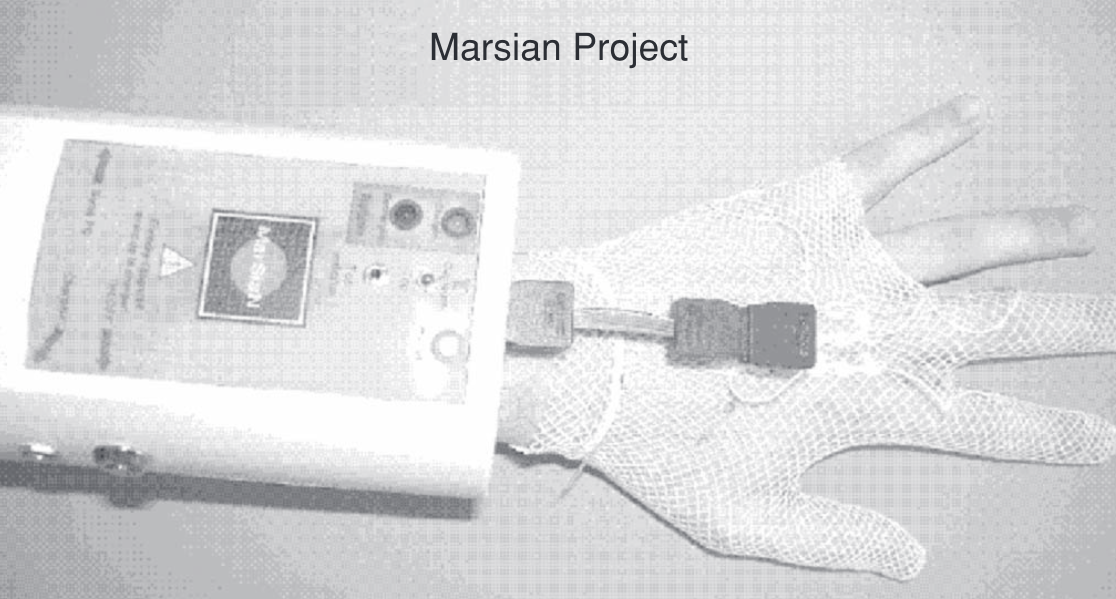
\includegraphics[width=0.8\textwidth]{img/rb-health.png}
            %\vspace{15pt}
            \caption{Ambulatório \Wearable.\ Uma instrumentação ambulatorial composta de roupas, luvas e dispositivo de pulso. Fonte: \citet{lmberis2007advanced}.}
            \label{fig:health}
        \end{figure}
    
        % ajuda em atividades
        Ao utilizar um dispositivo \wearable\ é possível também auxiliar e principalmente melhorar o desempenho de usuários nas mais diversas aplicações como por exemplo manutenção de aeronaves, assistência de navegação e inspeção veicular \citep{billinghurst1999wearable}.
        Um exemplo de interação que possível com o uso de \textit{smartphones} é exibido na Figura~\ref{fig:rb-routine} onde investigou-se o efeito de
        frequência de amostragem de auto-relatos de duas atividades de rotina, sendo elas sentar e andar.
        
        \begin{figure}[h] \centering
            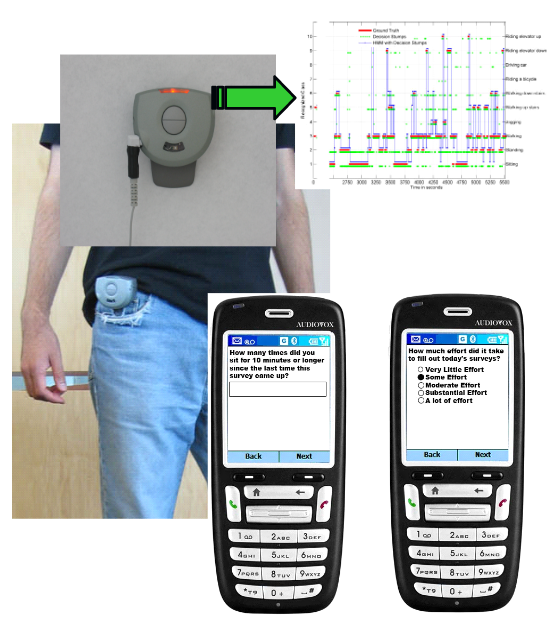
\includegraphics[width=0.7\textwidth]{img/rb-routine.png}
            \caption{Plataforma sensorial \wearable\ com a utilização de um telefone celular para interação. Fonte: \citet{Klasnja:2008:UWS:1409635.1409656}.}
            \label{fig:rb-routine}
        \end{figure}
        
        
        % industrial
        O estudo da computação \wearable\ no meio industrial foi motivado pela observação de que os sistemas móveis comuns não eram usáveis nas situações onde os usuários precisavam de foco em suas tarefas.
        Assim, a maioria das definições gerais de um sistema computacional industrial \wearable\ são definições funcionais de um sistema que pode ser usado em certo tempo, em qualquer lugar, e que não o distrai de suas interações com o mundo real para a realização de suas tarefas específicas \citep{lawo2007industrial}.
        Um exemplo é exibido na Figura~\ref{fig:industry}.
        
        \begin{figure}[h] \centering
            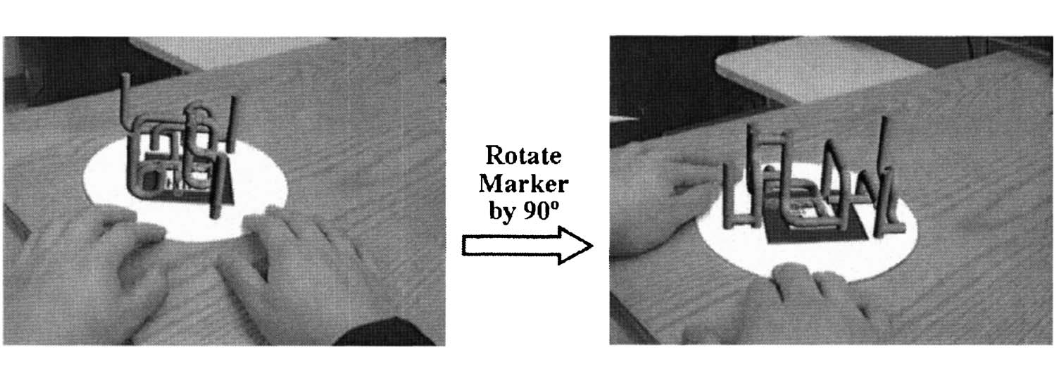
\includegraphics[width=0.97\textwidth]{img/rb-industry.png}
            \caption{\Wearable\ que permite a visualização e manuseio de projetos virtuais por meio de realidade aumentada. Fonte: \citet{dunston2005mixed}.}
            \label{fig:industry}
        \end{figure}
        
        % problemas
        \citet{patel2015wearable} aponta também quatro pontos que ainda representam problemas para o desenvolvimento e uso dos dispositivos \wearable\ e sua estabilização no cotidiano dos usuários.
        O primeiro é que uma pessoa deve ser motivada suficientemente para querer o dispositivo e estar disposta a utilizá-lo.
        Segundo, uma vez adquirido um dispositivo \wearable\ o usuário deve lembrar constantemente de utilizá-lo e ocasionalmente recarregá-lo.
        Terceiro empecilho é que a maioria dos dispositivos devem ser aptos a registrar de forma acurada os dados de seu ambiente utilizado sensores e aturadores.
        E por último, assumindo que a informação for lida com acurácia, os dados devem também serem apresentados ao usuários de forma compreensível para o seu entendimento das atividades realizadas e também motivando o uso contínuo do dispositivo.
        Dessa forma, mesmo que eles tenham grande potencial para facilitar a vida de usuários, a mudança não ocorre somente pelos dispositivos, necessitando uma grande demanda do hábito do usuário para seu uso.
        
        %cada vez mais usados
        Mas estudos como o de \citet{cornelius2014wearable} mostram que utilização de dispositivos eletrônicos inteligentes nas as redes de área corporal (do inglês \textit{body area network}) são cada vez mais usadas para monitoramento da saúde, assistência pessoal, entretenimento e automação residencial \citep{cornelius2014wearable}.
        
        
        % exemplo do crescimento 
        Um exemplo de seu potencial crescimento é no interesse cada vez mais de usuários tanto para uso quanto para desenvolvimento destes.
        \citet{merkouris2015introducing} em seu trabalho, avaliou experimentalmente a comparação dos benefícios da computação robótica e \wearable\ como plataforma meio no ensino de programação de dispositivos para crianças.
        Avaliaram atitudes e emoções dos estudantes antes e depois dos uso das plataformas de desenvolvimento e concluíram que utilizar computação obliqua como meio para aprendizagem de programação computadores é mais efetivo que o ensino de desenvolvimento para plataformas \textit{desktop} utilizadas geralmente.
        Citam também que mesmo que desenvolvimento para dispositivos \wearable\ não tenha sido tão motivador comparado com plataforma robótica, ainda sim apresentou-se mais interesse nas crianças que plataformas \textit{desktop}.
        
        
        % wearable e FPGA
        Além desses dispositivos, existe também desenvolvimentos de produtos \wearables\ que envolvem módulos em \hardware\ reconfiguráveis.
        Essa união permite que o \wearable\ utilize recursos de \hardware\ reconfigurável para suas tarefas além de poder se construído em totalmente nessa arquitetura sistêmica.
        O fruto deste produto entre essas tecnologias nos permite o alcançar maior poder de processamento com eficiência energética que processadores e microcontroladores tradicionais, desde que a aplicação corresponda bem às estruturas espaciais dos FPGAs \citep{Plessl2003}.
        \citet{demarco2011real} cita que enquanto adicionar a tecnologia de um FPGA em um projeto \wearable\ pode ter parecido complicado no \design,\ o FPGA fez com que fosse possível expandir facilmente as capacidades do sistema \wearable\ em momentos futuros.
        Um exemplo de conceito de uso é exibido na Figura~\ref{fig:rb-fpga} onde é descrito de forma esquemática um sistema para o monitoramento fetal domiciliar. 
        
        \begin{figure}[h] \centering
            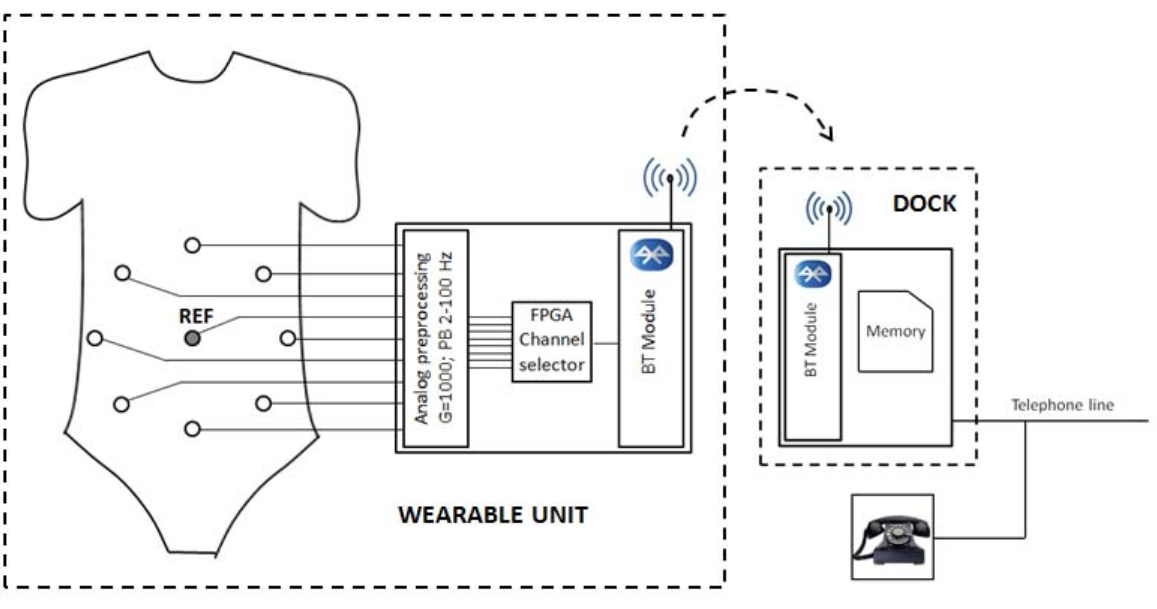
\includegraphics[width=0.97\textwidth]{img/rb-fpga.png}
            \caption{Monitoramento fetal domiciliar utilizando um FPGA e comunicação sem-fio. Fonte: \citet{fanelli2010prototype}.}
            \label{fig:rb-fpga}
        \end{figure}
        
        Caracteriza-se por uma unidade \wearable\ e uma estação de \textit{dock}. 
        Este é composto por um gravador colocado no na região do umbigo. 
        Um primeiro estágio opera um pré-processamento analógico com um FPGA extraindo a série, selecionando o canal com o melhor conteúdo de informação e os envia para o \textit{dock} através de uma conexão Bluetooth. 
        O \textit{dock} armazena as gravações em uma memória e as envia para o hospital através da linha telefônica.
        
        
        